\documentclass[conference]{IEEEtran}

\usepackage{cite}
\usepackage{amsmath,amssymb,amsfonts}
\usepackage{algorithmic}
\usepackage{graphicx}
\usepackage{textcomp}
\usepackage{xcolor}

\def\BibTeX{{\rm B\kern-.05em{\sc i\kern-.025em b}\kern-.08em
    T\kern-.1667em\lower.7ex\hbox{E}\kern-.125emX}}

\begin{document}

\title{Introduction to Remote Sensing and it's application}

\author{
    \IEEEauthorblockN{Ujjwol Kayastha}
    \IEEEauthorblockA{
        \textit{Department of Computer Science and Multimedia} \\
        \textit{Phoenix College of Management}\\
        \textit{Lincoln University}\\
        Maitidevi, Kathmandu, Nepal\\
        ujjwol.kayasthasp2022@pcmgmt.edu.np
    }
}

\maketitle

\begin{abstract}
    Remote sensing is a powerful tool that has revolutionized the way we observe and understand the Earth's surface. By using various sensors to detect and monitor physical characteristics of an area, remote sensing provides critical data for applications in environmental monitoring, urban planning, agriculture, and disaster management. This paper explores the principles of remote sensing, its technological advancements, and its wide range of applications.
\end{abstract}

\begin{IEEEkeywords}
    Remote Sensing, GIS, Urban Planning, Agriculture, Disaster Management
\end{IEEEkeywords}

\section{Introduction}
The seminar titled 'Introduction to Remote Sensing and its Applications' was organized by the Department of Computer Science and Multimedia at Phoenix College of Management, Lincoln University. The seminar was conducted by Dr. Bhoj Raj Ghimire, a renowned expert in the field of remote sensing and GIS. The seminar covered the basic principles of remote sensing, the technology used in remote sensing, and its applications in various fields such as agriculture, forestry, urban planning, and disaster management. This paper provides an overview of the seminar and highlights the key points discussed by Dr. Ghimire. He also discussed the importance of remote sensing in monitoring and managing natural resources, and how it can be used to address environmental challenges such as deforestation, climate change, and natural disasters.

\section{Remote Sensing}
Remote Sensing is the science of acquiring information about the Earth's surface without being in direct contact with it. It involves the use of sensors mounted on satellites, aircraft, drones, or ground-based platforms to capture data about the Earth's surface and atmosphere. The applications of remote sensing in agriculture are vast, from crop monitoring, land and forest mapping \cite{forestMapping}.

\begin{figure}
    \centering
    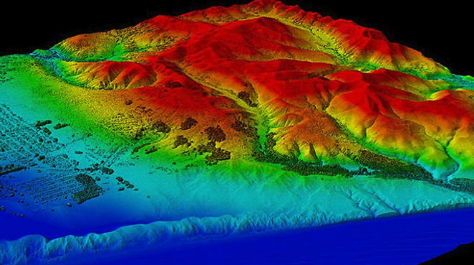
\includegraphics[width=\linewidth]{images/remote-sensing.png}
    \caption{A Lidar (Light Detection and Ranging) image created with data collected by NOAA's National Geodetic Survey}
    \label{fig:remote-sensing}
\end{figure}

\subsection{LiDAR}
LiDAR Lidar, which stands for Light Detection and Ranging, is a remote sensing method that uses light in the form of a pulsed laser to measure ranges (variable distances) to the Earth. These light pulses—combined with other data recorded by the airborne system — generate precise, three-dimensional information about the shape of the Earth and its surface characteristics. 
A lidar instrument principally consists of a laser, a scanner, and a specialized GPS receiver. Airplanes and helicopters are the most commonly used platforms for acquiring lidar data over broad areas. \cite{collis1970lidar}

\subsection{History of Remote Sensing}
The history of remote sensing dates back to the 19th century when the first aerial photographs were taken from hot air balloons. Since then, remote sensing technology has evolved significantly, with the development of satellite-based sensors, LiDAR technology, and other advanced imaging techniques. Today, remote sensing plays a crucial role in monitoring and managing natural resources, tracking environmental changes, and supporting decision-making in various fields. The earliest practices of modern remote sensing consisted of primitive photographs of the earth’s surface taken from tethered balloons for the purpose of topographic mapping in the 1840s.

\begin{figure}
    \centering
    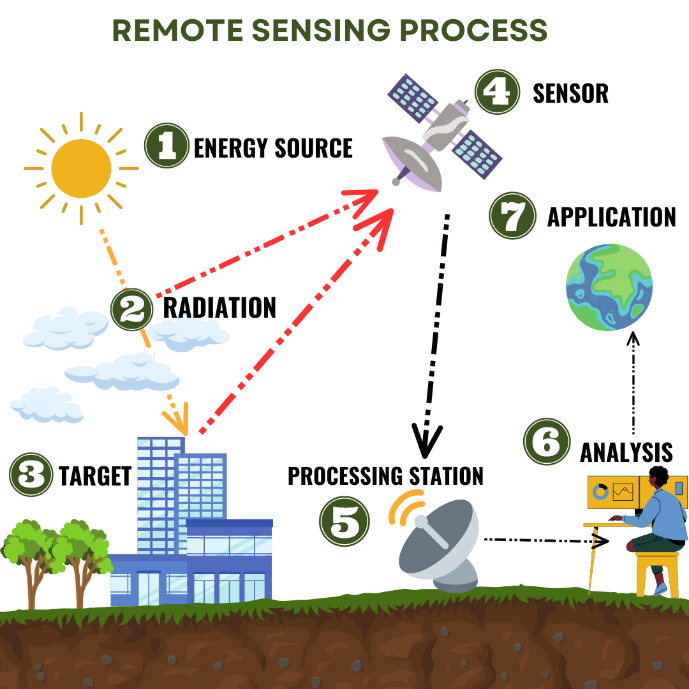
\includegraphics[width=\linewidth]{images/rs-process.png}
    \caption{Remote Sensing Process}
    \label{fig:remote-sensing-process}
\end{figure}

\subsection{Importance of Remote Sensing}
Remote sensing is a powerful tool that provides valuable data for a wide range of applications, including environmental monitoring, urban planning, agriculture, and disaster management. By using various sensors to detect and monitor physical characteristics of an area, remote sensing helps us understand the Earth's surface and its changes over time. This information is critical for making informed decisions about resource management, land use planning, and disaster response. Remote sensing technology has revolutionized the way we observe and understand the Earth's surface, providing critical data for applications in environmental monitoring, urban planning, agriculture, and disaster management. Remote sensing is also an unobstructive method, allowing users to collect data and perform data processing and GIS analysis offsite without disturbing the target area or object. Remote sensing, geographic information systems, and modeling have combined to produce a virtual explosion of growth in ecological investigations and applications that are explicitly spatial and temporal. \cite{cohen2004landsat} 

\section{Applications of Remote Sensing}
Remote sensing has a wide range of applications in various fields, including agriculture, forestry, urban planning, weather, disaster management, and environmental monitoring. Some of the key applications of remote sensing are as follows:

\subsection{Agriculture}
Remote sensing technology is widely used in agriculture for crop monitoring, yield prediction, and soil mapping. By analyzing satellite images and other remote sensing data, farmers can make informed decisions about planting, irrigation, and fertilization, leading to higher crop yields and reduced environmental impact.

\begin{figure}
    \centering
    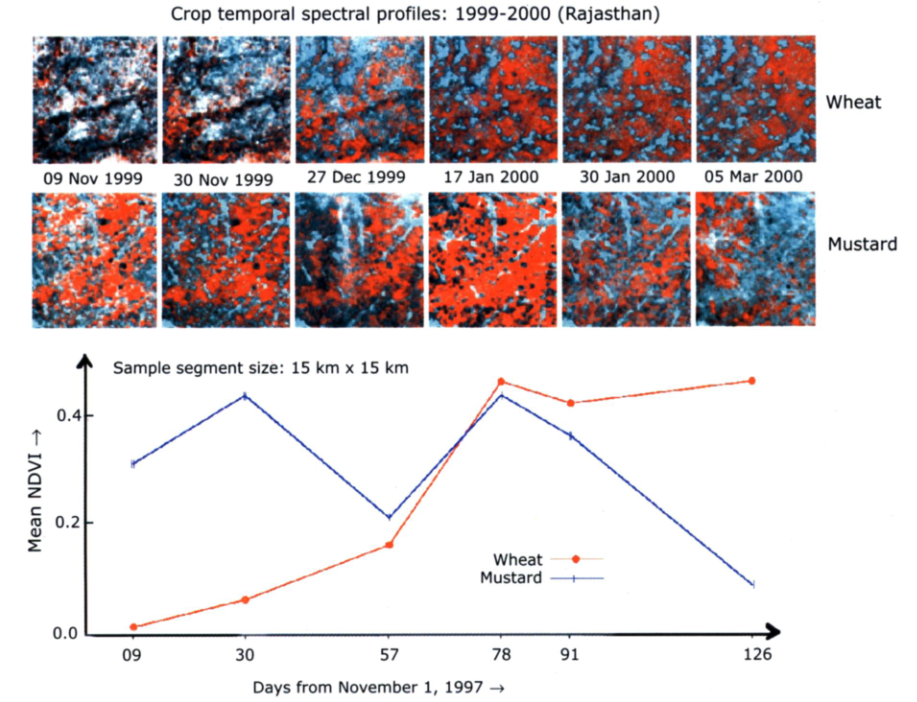
\includegraphics[width=\linewidth]{images/wheat-mustard.png}
    \caption{Multi temporal observations over agricultural region showing different growing pattern of wheat and mustard crops}
    \label{fig:application-agriculture}
\end{figure}
\subsubsection{Monitoring of vegetation cover}
Remote sensing technology is used to monitor vegetation cover and assess the health of crops. By analyzing satellite images and other remote sensing data, farmers can identify areas of stress, disease, or pest infestation and take corrective action to protect their crops. Many research experiments were done using aerial photographs and digital image processing techniques. But the field of remote sensing helps in reducing the amount of field data to be collected and improves the higher precision of estimates. \cite{shanmugapriya2019applications}

\subsection{Disaster Management}
Remote sensing plays a crucial role in disaster management by providing real-time data on natural disasters such as floods, earthquakes, and wildfires. By using satellite images and other remote sensing data, emergency responders can assess the extent of damage, identify areas at risk, and plan evacuation and rescue operations. Amarnath et al. (2017) have demonstrated the utility of less data intensive, but equally robust hydrodynamic models to develop flood extent maps in conjunction with freely available remote sensing imageries at different scales. \cite{Amarnath2024}

\subsection{Deep Learning in Remote Sensing}
Deep learning (DL) algorithms have seen a massive rise in popularity for remote-sensing image analysis over the past few years. Neural networks, the basis of deep learning (DL) algorithms, have been used in the remote sensing community for many years. However, prior to the development of DL, the remote-sensing community had shifted its focus from neural networks to support vector machine (SVM) and ensemble classifiers, e.g., random forest (RF), for image classification and other tasks (e.g. change detection). \cite{MA2019166} 

\subsection{Remote Sensing in Environment Monitoring}
Remote sensing has proven its usage in effective mapping/retrieval and monitoring of hydrological parameters such as precipitation, interception, soil moisture, surface runoff, surface water storage, surface water quality, evapotranspiration, change in terrestrial water storage, water level and river flow, etc. The basics of retrieval techniques, applications, modelling, validation and limitations are discussed along with the progress of each technique from optical to microwave remote sensing. \cite{Thakur2024}

\subsection{Urban Planning}
Swain et al. have demonstrated the utility of remote sensing data in urban planning and management. The study used remote sensing data to analyze land use and land cover changes in the city of Bhubaneswar, India, over a period of 20 years. The results showed significant changes in land use patterns, with a decrease in agricultural land and an increase in built-up areas. The study also highlighted the importance of remote sensing data in monitoring urban growth and planning for sustainable development. \cite{Swain2024}
Experts use remote sensing data to identify urban population growth patterns, analyze overcrowded areas, and make plans for infrastructure development such as public facilities, buildings, and roads.

\begin{figure}
    \centering
    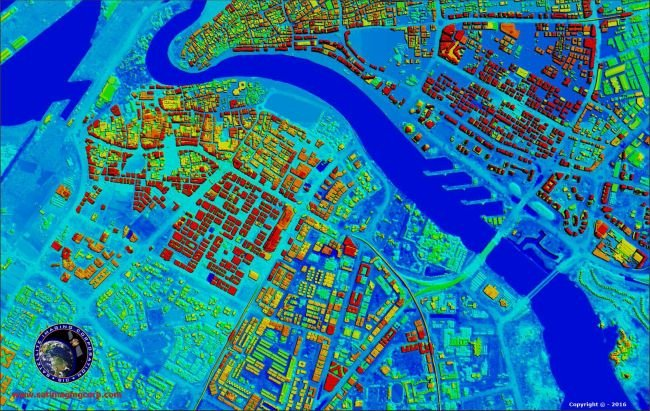
\includegraphics[width=\linewidth]{images/urbanplanning.jpg}
    \caption{Pleiades-1A Satellite Image – 2M DEM Urban Area in Dubai (2016)}
    \label{fig:urban-planning}
\end{figure}

\subsection{Water Security}
RS technology for water security and management are of diverse nature ranging from inventory of surface water bodies to more complex irrigation, groundwater exploration, snow-melt runoff forecast, flood forecasting, reservoir sedimentation, water quality monitoring, etc. 


\subsection{Community-centric Applications}
Initiatives towards community-centric applications harnessing the power of RS technology for the benefit of the community are gaining momentum. These applications include monitoring of water resources, land use, and land cover changes, disaster management, and climate change adaptation.

\subsection{Land Use Mapping and Monitoring}
Land use data represents how the landscape is being used for conservation, development, and agriculture. Remote sensing is used to map the land use pattern of large areas and monitor changes that occur over a particular period of time.
The satellite images provide a clear view of the land and help to determine the area which can be used for what purposes. This information is then used by regional planners and administrators to make policies for regional development.
\section{Conclusion}
Remote sensing has revolutionized the way we observe and understand the Earth's surface, providing critical data for a wide range of applications. From environmental monitoring to urban planning and disaster management, remote sensing technologies have proven to be indispensable. The seminar highlighted the importance of remote sensing in managing natural resources, monitoring environmental changes, and supporting decision-making processes. The continuous advancements in remote sensing technology promise even greater capabilities and applications in the future.

\section*{Acknowledgment}
I would like to thank Dr. Bhoj Raj Ghimire for his invaluable insights and guidance during the seminar. Special thanks to the Department of Computer Science and Multimedia at Phoenix College of Management for organizing the seminar. Gratitude is also extended to Lincoln University for its support and to all participants who contributed to the fruitful discussions.

\bibliographystyle{IEEEtran}
\bibliography{references}

\end{document}